\chapter*{Annexe 3 - Simulation \emph{SIMULINK}}
\addcontentsline{toc}{chapter}{Simulation \emph{SIMULINK}}
%\setcounter{section}{0}
% **********************************

%\label{Annex:SIMULINK_RE}
\lstset{
  language=Matlab,                	  % choose the language of the code
  basicstyle=\ttfamily,
  numbers=left,                   % where to put the line-numbers
  stepnumber=1,                   % the step between two line-numbers.
  numbersep=5pt,                  % how far the line-numbers are from the code
  backgroundcolor=\color{white},  % choose the background color. You must add \usepackage{color}
  commentstyle = \color{darkgreen},
  showspaces=false,               % show spaces adding particular underscores
  showstringspaces=false,         % underline spaces within strings
  showtabs=false,                 % show tabs within strings adding particular underscores
  tabsize=2,                      % sets default tabsize to 2 spaces
  captionpos=b,                   % sets the caption-position to bottom
  breaklines=true,                % sets automatic line breaking
  breakatwhitespace=true,         % sets if automatic breaks should only happen at whitespace
  %caption=exo1.m,                 % show the filename of files included with \lstinputlisting;
  literate={á}{{\'a}}1 {è}{{\`e}}1 {é}{{\'e}}1,
}
\section*{Modèles Non linéaire}\label{annex:modl_NL_SIMULINK}
\addcontentsline{toc}{section}{Modèles Non linéaire}
\begin{figure}
\centering
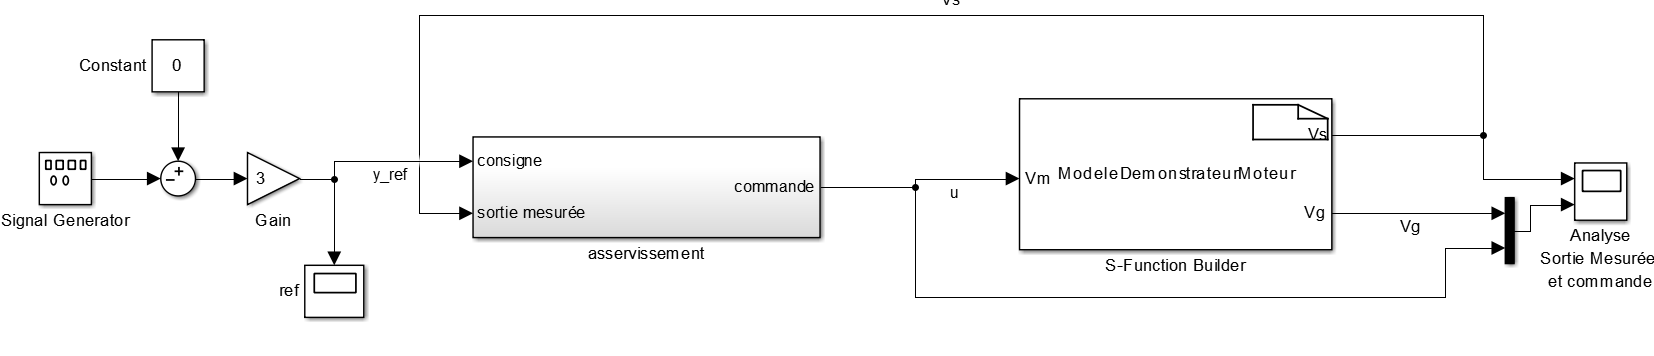
\includegraphics[width = \textwidth]{./annexes/annexe3/NL_RE_BlocEntier.png}
\caption{Schéma \emph{SIMULINK} complet de l'asservissement du modèle du moteur Non linéaire\label{fig:SIMULINK_NL_schema}}
\end{figure}

\begin{figure}
\centering
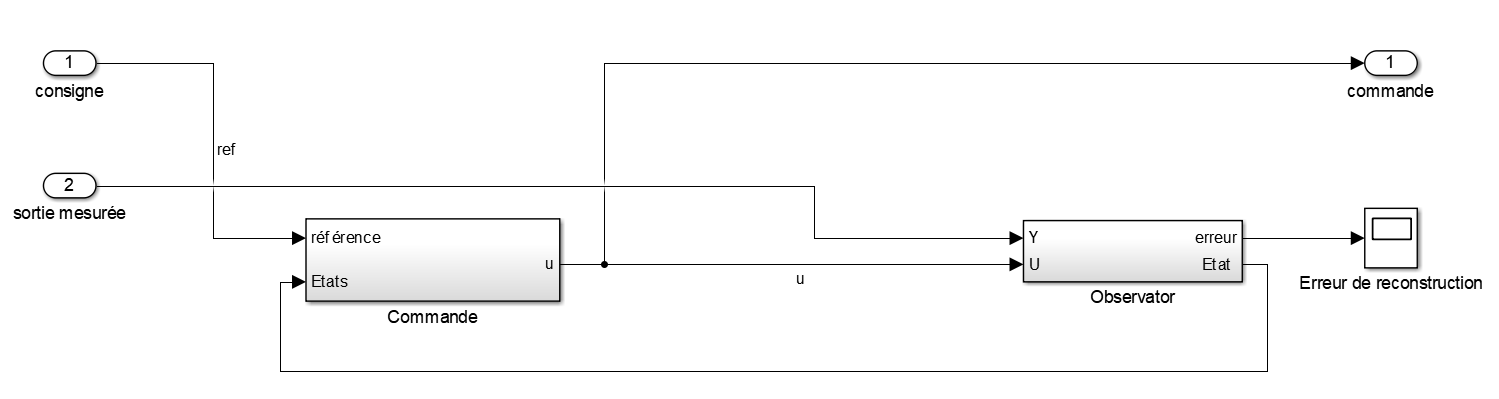
\includegraphics[width = \textwidth]{./annexes/annexe3/NL_RE_blocAsservissement.PNG}
\caption{Schéma \emph{SIMULINK} du \emph{sub-system} de commande\label{fig:SIMULINK_NL_subsystem_schema}}
\end{figure}

\begin{figure}
\centering
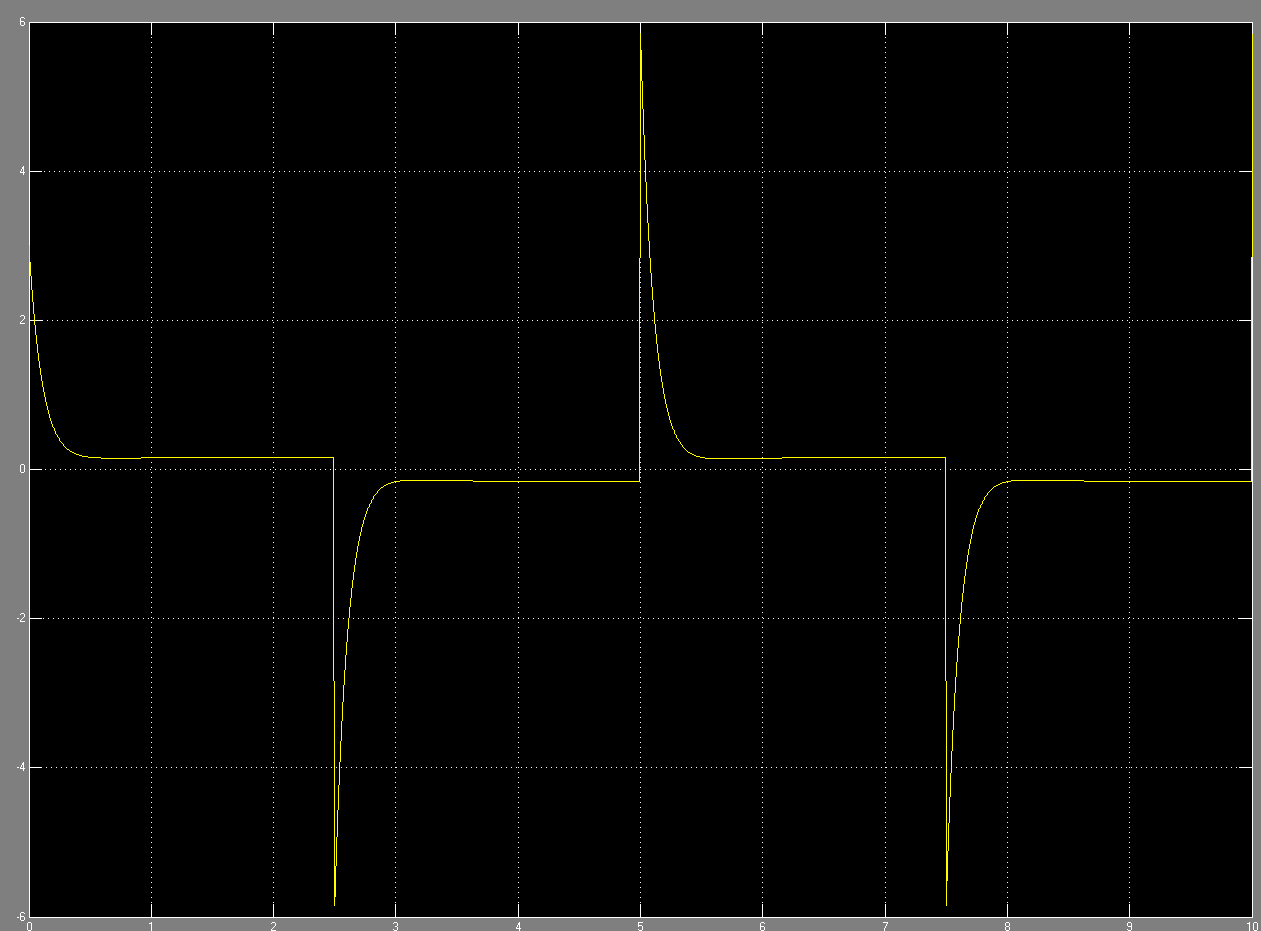
\includegraphics[width = .9\textwidth]{./annexes/annexe3/NL_erreur-Consigne_Vs_RE.png}
\caption{Mesure de simulation de l'erreur $\epsilon$ entre la référence et la sortie $V_s$ du modèle Non linéaire\label{fig:SIMULINK_NL_erreur_reponse}}
\end{figure}

\begin{figure}
\centering
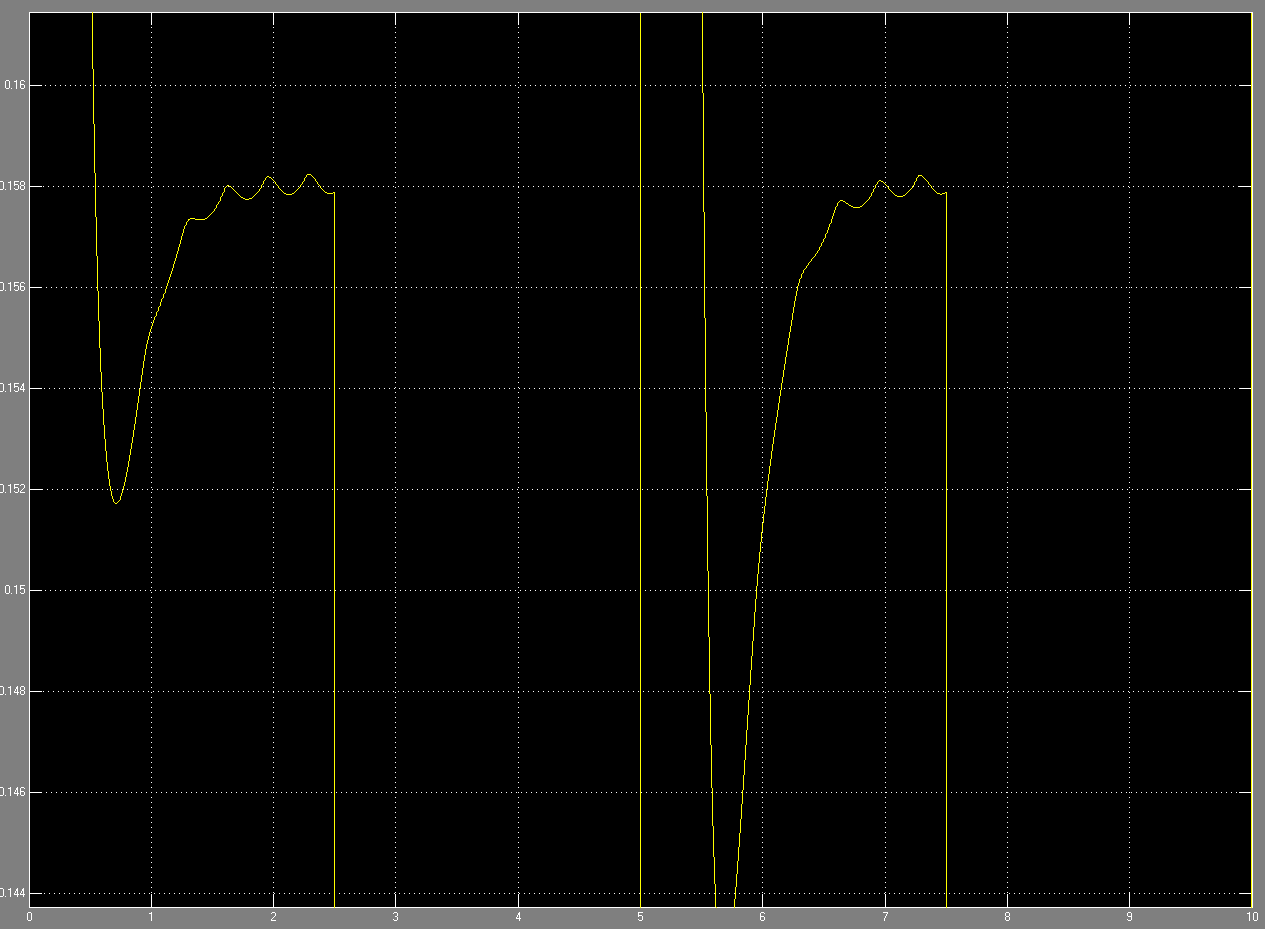
\includegraphics[width = .9\textwidth]{./annexes/annexe3/NL_erreur-Consigne_Vs_RE_zoom.png}
\caption{Mesure de simulation de l'erreur $\epsilon$ du modèle Non linéaire centré sur l'axe des ordonnées en $[0.144; 0.16].$\label{fig:SIMULINK_NL_erreur_reponse_zoom}}	
\end{figure}


>>>>>>> RapportChap4-2

